\documentclass[11pt]{article} % use larger type; default would be 10pt

\usepackage{tikz}
\usetikzlibrary{calc}

        \newcommand\degree[0]{^{\circ}}

\title{Play with TikZ}
\author{Just Us}
%\date{} % Activate to display a given date or no date (if empty),
         % otherwise the current date is printed 

\begin{document}
\maketitle

\section{Triangles}


rotate and translate triangles 
\begin{tikzpicture}
\coordinate (A) at (0,0 );
\coordinate (B) at (1.3,1.8);
\coordinate (C) at (4.5,.25);


\filldraw[black] (A) circle (.2pt) node[anchor=north east, xshift=0, yshift=0]{$A$};
\filldraw[black] (B) circle (.2pt) node[anchor=south , xshift=0, yshift=0]{$B$};
\filldraw[black] (C) circle (.2pt) node[anchor= west, xshift=0, yshift=0]{$C$};

\filldraw[ black, shift={(7 cm, 3 cm)}, rotate=-65]  (0,0) circle (.2pt) node[anchor=east, xshift=0, yshift=0]{$D$};
\filldraw[black, shift={(7 cm, 3 cm)}, rotate=-65] (1.3,1.8) circle (.2pt) node[anchor=west , xshift=0, yshift=0]{$E$};
\filldraw[black, shift={(7 cm, 3 cm)}, rotate=-65] (4.5,.25) circle (.2pt) node[anchor=north west, xshift=0, yshift=0]{$F$};

\draw (A)--(B) node[left, midway, xshift=-3,yshift=1] {\color{blue}$c$};
\draw (B)--(C) node[right, midway, xshift=3,yshift=2] {\color{blue}$a$};
\draw (A)--(C) node[below, midway, yshift=-3] {\color{blue}$b$};

\draw[black, shift={(7 cm, 3 cm)}, rotate=-65]  (0,0)--(1.3,1.8) node[above, midway, xshift=0,yshift=3] {\color{blue}$f$};
\draw[black, shift={(7 cm, 3 cm)}, rotate=-65]  (1.3,1.8)--(4.5,.25) node[right, midway, xshift=3,yshift=2] {\color{blue}$d$};
\draw[black, shift={(7 cm, 3 cm)}, rotate=-65]  (0,0)--(4.5,.25) node[left, midway, xshift=-2, yshift=-3] {\color{blue}$e$};

\end{tikzpicture}
\newline


congruent triangles
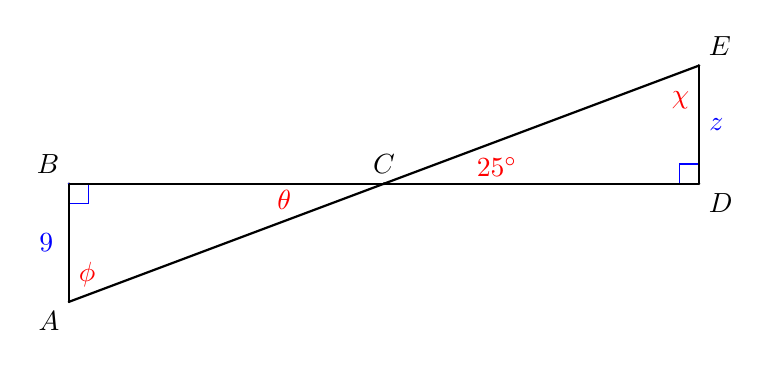
\begin{tikzpicture}
\coordinate (A) at (-4,-1.5 );
\coordinate (B) at (-4,0);
\coordinate (C) at(0,0);
\coordinate (D) at (4,0);
\coordinate (E) at(4,1.5);

\filldraw[black] (A) circle (.2pt) node[anchor=north east, xshift=0, yshift=0]{$A$};
\filldraw[black] (A) circle (.2pt) node[anchor=south west, xshift=0, yshift=2]{\color{red}$\phi$};

\filldraw[black] (B) circle (.2pt) node[anchor=south east, xshift=0, yshift=0]{$B$};
\draw[blue] (B) rectangle +(0.25,-0.25);

\filldraw[black] (C) circle (.2pt) node[anchor=south, xshift=0, yshift=0]{$C$};
\filldraw[black] (C) circle (.2pt) node[anchor=north east, xshift=-30, yshift=1]{\color{red}$\theta$};
\filldraw[black] (C) circle (.2pt) node[anchor=south west, xshift=30, yshift=-1]{\color{red}$25\degree$};

\filldraw[black] (D) circle (.2pt) node[anchor=north west, xshift=0, yshift=0]{$D$};
\draw[blue] (D) rectangle +(-0.25,0.25);


\filldraw[black] (E) circle (.2pt) node[anchor=south west, xshift=0, yshift=0]{$E$};
\filldraw[black] (E) circle (.2pt) node[anchor=north east, xshift=0, yshift=-6]{\color{red}$\chi$};

\draw[black,  thick] (A) -- (B) node [left, midway, xshift=-2] {\color{blue}9};
\draw[black,  thick] (B) --( D)  ;
\draw[black,  thick] (A) -- (E)  ;
\draw[black, thick] (E) -- (D) node[right, midway]{\color{blue}$z$};

\end{tikzpicture}
\newline


1.2 Exercise 1
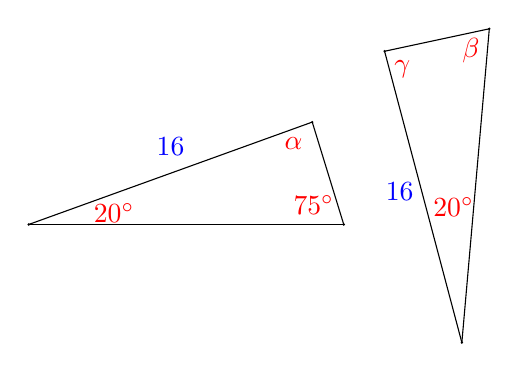
\begin{tikzpicture}
\coordinate (A) at (0,0 );
\coordinate (B) at (4,0);
\coordinate (C) at (3.6,1.3);


\filldraw[black] (A) circle (.2pt) node[anchor=south west, xshift=20, yshift=-3]{\color{red}$20\degree$};
\filldraw[black] (B) circle (.2pt) node[anchor=south east, xshift=0, yshift=0]{\color{red}$75\degree$};
\filldraw[black] (C) circle (.2pt) node[anchor= north east, xshift=0, yshift=-2]{\color{red}$\alpha$};

\filldraw[ black, shift={(5.5 cm, -1.5 cm)}, rotate=85]  (0,0) circle (.2pt) node[anchor=south, xshift=-3, yshift=42]{\color{red}$20\degree$};
\filldraw[black, shift={(5.5 cm, -1.5 cm)}, rotate=85] (4,0) circle (.2pt) node[anchor=north east , xshift=0, yshift=0]{\color{red}$\beta$};
\filldraw[black, shift={(5.5 cm, -1.5 cm)}, rotate=85] (3.6,1.3) circle (.2pt) node[anchor=north west, xshift=0, yshift=0]{\color{red}$\gamma$};


\draw (A)--(B) ;
\draw (B)--(C) ;
\draw (A)--(C) node[above, midway, yshift=3] {\color{blue}$16$};

\draw[black, shift={(5.5 cm, -1.5 cm)}, rotate=85]  (0,0)--(4,0);
\draw[black, shift={(5.5 cm, -1.5 cm)}, rotate=85]  (4,0)--(3.6,1.3) ;
\draw[black, shift={(5.5 cm, -1.5 cm)}, rotate=85]  (0,0)--(3.6,1.3) node[left, midway, xshift=0, yshift=2] {\color{blue}$16$};

\end{tikzpicture}
\newline


Example 2
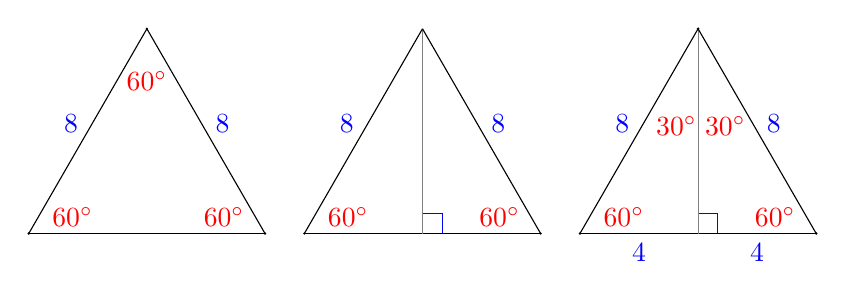
\begin{tikzpicture}
\coordinate (A) at (0,0);
\coordinate (B) at (3,0);
\coordinate(C) at (1.5,2.6);

\filldraw[black] (A) circle (.2pt) node[anchor=south west, xshift=5, yshift=-1]{\color{red}$60\degree$};
\filldraw[black] (B) circle (.2pt) node[anchor=south east, xshift=-4, yshift=-1]{\color{red}$60\degree$};
\filldraw[black] (C) circle (.2pt) node[anchor=north , yshift=-12]{\color{red}$60\degree$};

\draw[black] (A) --  (B) ;
\draw[black] (A) --  (C) node [above left, midway,yshift=-4] {\color{blue}$8$};
\draw[black] (C) --  (B) node [above right, midway,yshift=-4] {\color{blue}$8$};

\coordinate (A2) at (3.5,0);
\coordinate (B2) at (6.5,0);
\coordinate(C2) at (5,2.6);
\coordinate(D2) at (5,0);

\filldraw[black] (A2) circle (.2pt) node[anchor=south west, xshift=5, yshift=-1]{\color{red}$60\degree$};
\filldraw[black] (B2) circle (.2pt) node[anchor=south east, xshift=-4, yshift=-1]{\color{red}$60\degree$};

\draw[blue] (D2) rectangle +(.25,.25);
\draw[black] (A2) --  (B2) ;
\draw[gray] (C2) --  (D2) ;
\draw[black] (A2) --  (C2) node [above left, midway,yshift=-4] {\color{blue}$8$};
\draw[black] (C2) --  (B2) node [above right, midway,yshift=-4] {\color{blue}$8$};

\coordinate (A3) at (7,0);
\coordinate (B3) at (10,0);
\coordinate(C3) at (8.5,2.6);
\coordinate(D3) at (8.5,0);

\filldraw[black] (A3) circle (.2pt) node[anchor=south west, xshift=5, yshift=-1]{\color{red}$60\degree$};
\filldraw[black] (B3) circle (.2pt) node[anchor=south east, xshift=-4, yshift=-1]{\color{red}$60\degree$};
\filldraw[black] (C3) circle (.2pt) node[anchor=north east, xshift=3, yshift=-28]{\color{red}$30\degree$};
\filldraw[black] (C3) circle (.2pt) node[anchor=north west, xshift=-1, yshift=-28]{\color{red}$30\degree$};

\draw[blue] (D3) rectangle +(.25,.25);
\draw[black] (A3) --  (D3)  node [below, midway,yshift=0] {\color{blue}$4$};
\draw[black] (B3) --  (D3)  node [below, midway,yshift=0] {\color{blue}$4$};
\draw[gray] (C3) --  (D3) ;
\draw[black] (A3) --  (C3) node [above left, midway,yshift=-4] {\color{blue}$8$};
\draw[black] (C3) --  (B3) node [above right, midway,yshift=-4] {\color{blue}$8$};

\end{tikzpicture}
\newline



Exercise 2
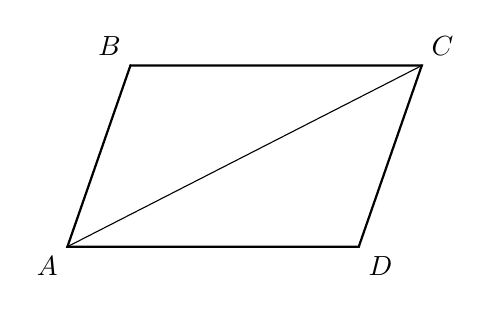
\begin{tikzpicture}
\coordinate (A) at (0,0);
\coordinate (B) at (.8,2.3);
\coordinate(C) at (4.5,2.3);
\coordinate (D) at (3.7,0);

\filldraw[black] (A) circle (.2pt) node[anchor=north east]{$A$};
\filldraw[black] (B) circle (.2pt) node[anchor=south east, xshift=0]{$B$};
\filldraw[black] (C) circle (.2pt) node[anchor=south west]{$C$};
\filldraw[black] (D) circle (.2pt) node[anchor=north west]{$D$};
\draw[black,  thick] (A) -- (B) --( C) --(D)-- cycle;
\draw[black] (A) --  (C);

\end{tikzpicture}
\newline


Similar triangles
%next time put O at the origin, then define A, B, C etc.
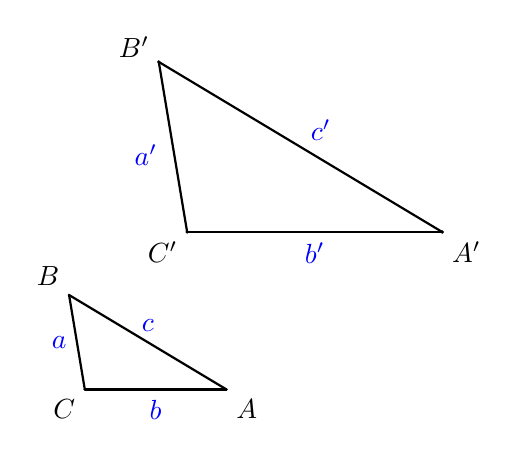
\begin{tikzpicture}
\coordinate (A) at (1.8,0);
\coordinate (B) at (-.2,1.2);
\coordinate(C) at (0,0);

\filldraw[black] (A) circle (.2pt) node[anchor=north west]{$A$};
\filldraw[black] (B) circle (.2pt) node[anchor=south east, xshift=0]{$B$};
\filldraw[black] (C) circle (.2pt) node[anchor=north east]{$C$};

%\draw[black,  thick] (A) -- (B) --( C) -- cycle;
\draw[black,  thick] (A) --  (C) node[below, midway] {$\color{blue}b$};
\draw[black,  thick] (A) --  (B) node[above, midway] {$\color{blue}c$};
\draw[black,  thick] (B) --  (C) node[left, midway] {$\color{blue}a$};

\filldraw[black, shift={(1.3 cm, 2 cm)},scale=1.8] (1.8,0) circle (.2pt) node[anchor=north west]{$A'$};
\filldraw[black, shift={(1.3 cm, 2 cm)},scale=1.8] (-.2,1.2) circle (.2pt) node[anchor=south east, yshift=-2]{$B'$};
\filldraw[black, shift={(1.3 cm, 2 cm)},scale=1.8] (0,0) circle (.2pt) node[anchor=north east]{$C'$};


\draw[black,  thick, shift={(1.3 cm, 2 cm)},scale=1.8]  (0,0)--(1.8,0) node[below, midway, xshift=0,yshift=0] {$\color{blue}b '$};
\draw[black,  thick, shift={(1.3 cm, 2 cm)}, scale=1.8]  (1.8,0)--(-.2,1.2) node[right, midway, xshift=0,yshift=6] {$\color{blue}c '$};
\draw[black,  thick, shift={(1.3 cm, 2 cm)}, scale=1.8]  (0,0)--(-.2,1.2) node[left, midway, xshift=-2, yshift=-3] {$\color{blue}a '$};

\end{tikzpicture}
\newline




Similar triangles
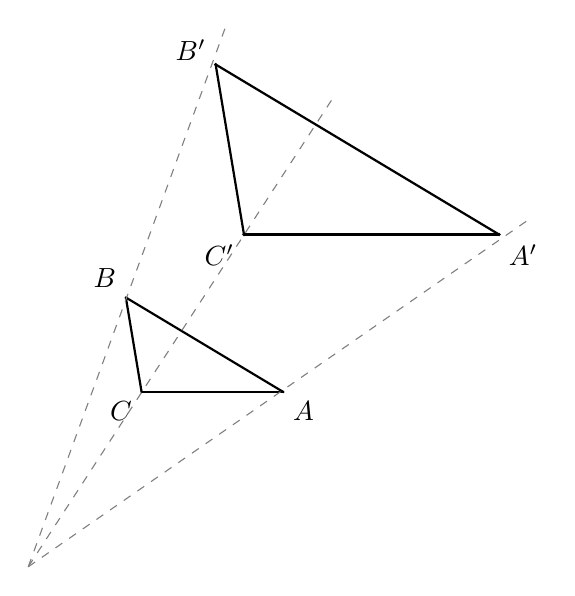
\begin{tikzpicture}
\coordinate (A) at (1.8,0);
\coordinate (B) at (-.2,1.2);
\coordinate(C) at (0,0);
\coordinate(O) at (-1.44,-2.22);


\filldraw[black] (A) circle (.2pt) node[anchor=north west]{$A$};
\filldraw[black] (B) circle (.2pt) node[anchor=south east, xshift=0]{$B$};
\filldraw[black] (C) circle (.2pt) node[anchor=north east]{$C$};

\draw[black,  thick] (A) --  (C);
\draw[black,  thick] (A) --  (B) ;
\draw[black,  thick] (B) --  (C) ;

\filldraw[black, shift={(1.3 cm, 2 cm)},scale=1.8] (1.8,0) circle (.2pt) node[anchor=north west]{$A'$};
\filldraw[black, shift={(1.3 cm, 2 cm)},scale=1.8] (-.2,1.2) circle (.2pt) node[anchor=south east, yshift=-2]{$B'$};
\filldraw[black, shift={(1.3 cm, 2 cm)},scale=1.8] (0,0) circle (.2pt) node[anchor=north east]{$C'$};


\draw[black,  thick, shift={(1.3 cm, 2 cm)},scale=1.8]  (0,0)--(1.8,0) ;
\draw[black,  thick, shift={(1.3 cm, 2 cm)}, scale=1.8]  (1.8,0)--(-.2,1.2) ;
\draw[black,  thick, shift={(1.3 cm, 2 cm)}, scale=1.8]  (0,0)--(-.2,1.2) ;

\draw[gray, dashed] (O) --  +(3.9,6);
\draw[gray, dashed] (O) --    +(2.5,6.84) ;
\draw[gray, dashed] (O) --    +(6.4,4.44) ;

\end{tikzpicture}
\newline


Example 3a
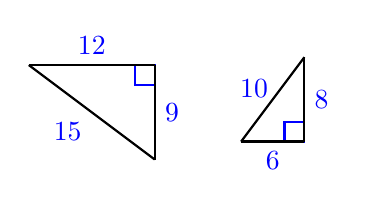
\begin{tikzpicture}
\coordinate (A) at (0,0);
\coordinate (B) at (1.6,0);
\coordinate(C) at (1.6,-1.2);

\draw[blue, thick] (B) rectangle +(-0.25,-0.25);

\draw[black,  thick] (A) --  (C) node[below left, midway] {\color{blue}$15$};
\draw[black,  thick] (A) --  (B) node[above, midway] {\color{blue}$12$} ;
\draw[black,  thick] (B) --  (C) node[right, midway] {\color{blue}$9$};


\draw[blue,  thick, shift={(3.5 cm, .1 cm)},scale=0.67, rotate=-90]  (1.6,0) rectangle +(-0.375,-0.375);
\draw[black,  thick, shift={(3.5 cm, .1 cm)},scale=0.67, rotate=-90]  (0,0)--(1.6,0) node [right, midway] {\color{blue}$8$};
\draw[black,  thick, shift={(3.5 cm, .1 cm)},scale=0.67, rotate=-90]   (1.6,0)--(1.6,-1.2) node [below, midway] {\color{blue}$6$};
\draw[black,  thick, shift={(3.5 cm, .1 cm)},scale=0.67, rotate=-90]   (0,0)--(1.6,-1.2) node [above left, midway, xshift=2, yshift=-3] {\color{blue}$10$};

\end{tikzpicture}
\newline



Example 3b
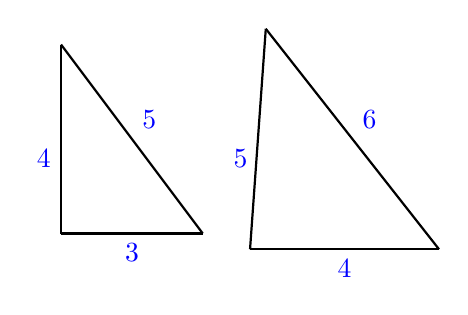
\begin{tikzpicture}

\coordinate (A) at (0,0);
\coordinate (B) at (1.8,0);
\coordinate(C) at (0,2.4);

\draw[black,  thick] (A) --  (C) node[below left, midway] {\color{blue}$4$};
\draw[black,  thick] (A) --  (B) node[below, midway] {\color{blue}$3$} ;
\draw[black,  thick] (B) --  (C) node[above right, midway] {\color{blue}$5$};


\coordinate (A2) at (2.4,-0.2);
\coordinate (B2) at (4.8,-0.2);
\coordinate(C2) at (2.6,2.6);

\draw[black,  thick] (A2) --  (C2) node[below left, midway] {\color{blue}$5$};
\draw[black,  thick] (A2) --  (B2) node[below, midway] {\color{blue}$4$} ;
\draw[black,  thick] (B2) --  (C2) node[above right, midway] {\color{blue}$6$};

\end{tikzpicture}
\newline


Example 3c
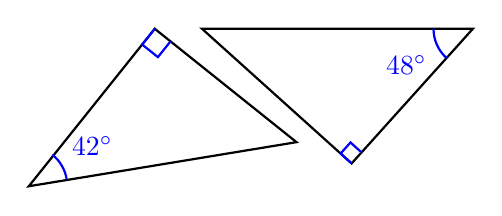
\begin{tikzpicture}

\coordinate (A) at (0,0);
\coordinate (B) at (-1.6,-2);
\coordinate (C) at (1.8,-1.44);

\draw[black,  thick] (A) --  (B) -- (C) -- cycle ;
\draw[blue,  thick]  (A) -- ++(-.16,-.2) -- ++(.2,-.16) -- ++(.16,.2);
\draw[blue, thick] (-1.3,-1.6) arc ({atan(1.25)}:{atan(.1647}:.5) node [above right, midway] {$42\degree$};


\coordinate (A2) at (2.5,-1.71);
\coordinate (B2) at (.6,0);
\coordinate (C2) at (4.04,0);

\draw[black,  thick] (A2) --  (B2) -- (C2) -- cycle ;
\draw[blue,  thick]  (A2) -- ++(-.14,.126) -- ++(.126,.14) -- ++(.14,-.126);
\draw[blue, thick] (3.54,0) arc (180:228:.5) node [below left, midway] {$48\degree$};

\end{tikzpicture}
\newline


Exercise 3a
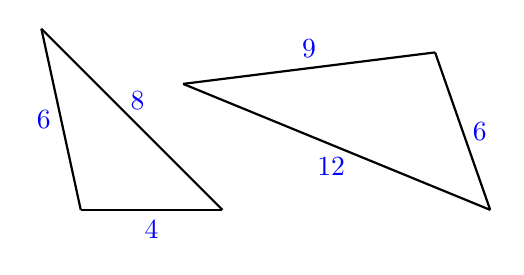
\begin{tikzpicture}

\coordinate (A) at (0,0);
\coordinate (B) at (-.5,2.3);
\coordinate (C) at (1.8,0);

%\draw[black,  thick] (A) --  (B) -- (C) -- cycle ;
\draw[black, thick] (A) --  (B) node[left,midway] {\color{blue}$6$} ;
\draw[black, thick] (A)  -- (C) node[below,midway] {\color{blue}$4$} ;
\draw[black, thick] (B) -- (C) node[above ,midway,xshift=2] {\color{blue}$8$} ;


\coordinate (A2) at (4.5,2);
\coordinate (B2) at (5.2,0);
\coordinate (C2) at (1.3,1.6);

%\draw[black,  thick] (A2) --  (B2) -- (C2) -- cycle ;
\draw[black, thick] (A2) --  (B2) node[right,midway] {\color{blue}$6$} ;
\draw[black, thick] (A2)  -- (C2) node[above,midway] {\color{blue}$9$} ;
\draw[black, thick] (B2) -- (C2) node[below,midway,xshift=-2] {\color{blue}$12$} ;

\end{tikzpicture}
\newline



Exercise 3b
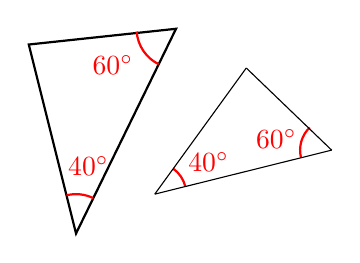
\begin{tikzpicture}

\coordinate (A) at (0,0);
\coordinate (B) at (-.6,2.4);
\coordinate (C) at (1.27,2.6);

\draw[black,  thick] (A) --  (B) -- (C) -- cycle ;
\draw[red, thick] (-.121,.485) arc (104:64:0.5) node [above, midway, xshift=3, yshift=3] {\color{red}$40\degree$};
\draw[red, thick] (1.05,2.15) arc (244:184:0.5) node [below left, midway, xshift=0, yshift=2] {\color{red}$60\degree$};

\draw[red, thick,shift={(1 cm, .5 cm)}, rotate=-50, scale=.8] (-.121,.485) arc (104:64:0.5) node [above, midway, xshift=10, yshift=-2] {\color{red}$40\degree$};
\draw[red, thick, shift={(1 cm, .5 cm)}, rotate=-50, scale=.8] (1.05,2.15) arc (244:184:0.5) node [below left, midway, xshift=2, yshift=8] {\color{red}$60\degree$};

\draw[black, shift={(1 cm, .5 cm)}, rotate=-50, scale=.8]  (0,0)--(-.6,2.4);
\draw[black, shift={(1 cm, .5 cm)}, rotate=-50, scale=.8]  (-.6,2.4)--(1.27,2.6) ;
\draw[black, shift={(1 cm, .5 cm)}, rotate=-50, scale=.8]  (0,0)--(1.27,2.6) ;

\end{tikzpicture}
\newline




Example 4
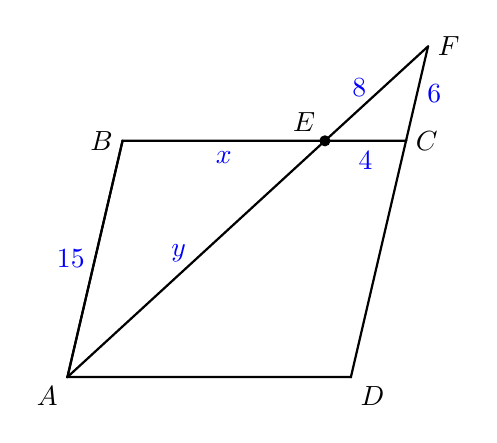
\begin{tikzpicture}

\coordinate (A) at (0,0);
\coordinate (B) at (.7,3);
\coordinate (C) at (4.3,3);
\coordinate (D) at (3.6,0);
\coordinate (E) at (3.27,3);
\coordinate (F) at (4.58,4.2);

\draw[black,  thick] (A) --  (B) -- (C) -- (D) -- cycle ;
\draw[black,  thick] (F) -- (C) node[right, midway] {\color{blue}$6$} ;
\draw[black,  thick] (F) -- (E) node[left, midway, yshift=2] {\color{blue}$8$} ;
\draw[black,  thick] (A) -- (E) node[left, midway,yshift=2] {\color{blue}$y$} ;
\draw[black,  thick] (C) -- (E) node[below, midway] {\color{blue}$4$} ;
\draw[black,  thick] (B) -- (E) node[below, midway] {\color{blue}$x$} ;
\draw[black,  thick] (B) -- (A) node[left, midway] {\color{blue}$15$} ;

\filldraw[black] (A) circle (.2pt) node[anchor=north east]{$A$};
\filldraw[black] (B) circle (.2pt) node[anchor= east]{$B$};
\filldraw[black] (C) circle (.2pt) node[anchor=west]{$C$};
\filldraw[black] (D) circle (.2pt) node[anchor=north west]{$D$};
\filldraw[black] (E) circle (1.8pt) node[anchor=south east]{$E$};
\filldraw[black] (F) circle (.2pt) node[anchor= west]{$F$};

\end{tikzpicture}
\newline





Example 5
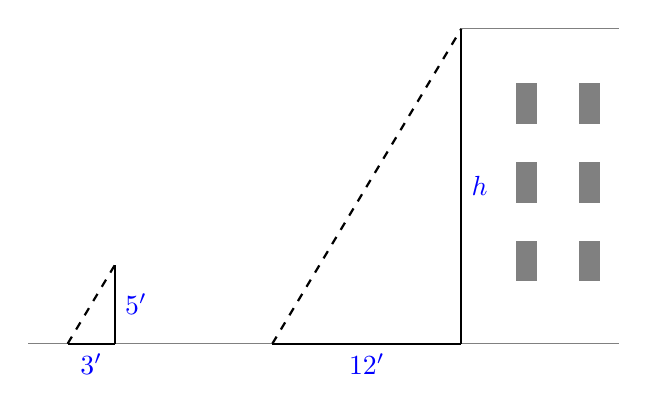
\begin{tikzpicture}

\coordinate (A) at (0,0);
\coordinate (B) at (.6,1);
\coordinate (C) at (.6,0);
\coordinate (D) at (2.6,0);
\coordinate (E) at (5,4);
\coordinate (F) at (5,0);

\draw[gray] (-.5,0) -- (7,0);
\draw[gray] (5,4) -- (7,4);
\draw[black,  thick, dashed] (A) -- (B)  ;
\draw[black,  thick] (A) -- (C) node[below, midway, yshift=0] {\color{blue}$3'$} ;
\draw[black,  thick] (B) -- (C) node[right, midway, yshift=0] {\color{blue}$5'$} ;

\draw[black,  thick, dashed] (D) -- (E)  ;
\draw[black,  thick] (D) -- (F) node[below, midway, yshift=0] {\color{blue}$12'$} ;
\draw[black,  thick] (E) -- (F) node[right, midway, yshift=0] {\color{blue}$h$} ;

\filldraw[gray] (5.7, .8) rectangle +(.25,.5);
\filldraw[gray] (5.7, 1.8) rectangle +(.25,.5);
\filldraw[gray] (5.7, 2.8) rectangle +(.25,.5);
\filldraw[gray] (6.5, .8) rectangle +(.25,.5);
\filldraw[gray] (6.5, 1.8) rectangle +(.25,.5);
\filldraw[gray] (6.5, 2.8) rectangle +(.25,.5);

\end{tikzpicture}
\newline



Example 6
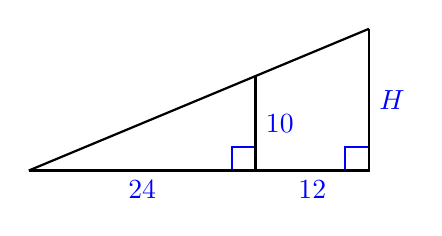
\begin{tikzpicture}[scale=1.2]

\coordinate (A) at (0,0);
\coordinate (B) at (2.4,1);
\coordinate (C) at (2.4,0);
\coordinate (D) at (3.6,1.5);
\coordinate (E) at (3.6,0);

\draw[blue, thick] (C) rectangle +(-.25, .25);
\draw[blue, thick] (E) rectangle +(-.25, .25);
\draw[black,  thick] (A) --  (C) node[below,midway] {\color{blue}$24$} ;
\draw[black,  thick] (B) -- (C) node[right, midway] {\color{blue}$10$} ;
\draw[black,  thick] (C) -- (E) node[below, midway, yshift=0] {\color{blue}$12$} ;
\draw[black,  thick] (D) -- (E) node[right, midway,yshift=0] {\color{blue}$H$} ;
\draw[black,  thick] (A) -- (D)  ;

\end{tikzpicture}
\newline


Example 6 Solution
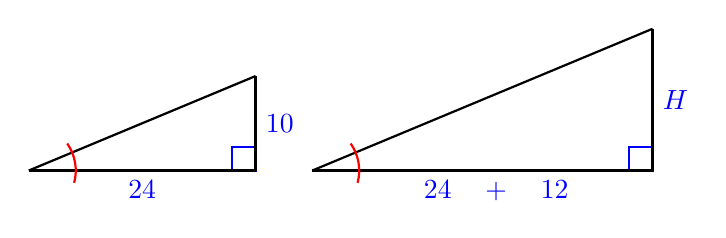
\begin{tikzpicture}[scale=1.2]

\coordinate (A) at (0,0);
\coordinate (B) at (2.4,1);
\coordinate (C) at (2.4,0);
\coordinate (D) at (6.6,1.5);
\coordinate (E) at (6.6,0);
\coordinate (A2) at (3,0);

\draw[blue, thick] (C) rectangle +(-.25, .25);
\draw[blue, thick] (E) rectangle +(-.25, .25);
\draw[black,  thick] (A) -- (B)  ;
\draw[black, thick] (A) --  (C) node[below,midway] {\color{blue}$24$};
\draw[black,  thick] (B) -- (C) node[right, midway] {\color{blue}$10$} ;

\draw[red,thick] (0.48,-0.13) arc (-15:35:0.5);

\draw[black,  thick] (A2) -- (E) node[below, midway, xshift=5] {\color{blue}$24~~~+~~~12$} ;
\draw[black,  thick] (D) -- (E) node[right, midway,yshift=0] {\color{blue}$H$} ;
\draw[black,  thick] (A2) -- (D)  ;
\draw[red,thick] (3.48,-0.13) arc (-15:35:0.5);

\end{tikzpicture}
\newline




Exercise 6 exists in pdf textbook
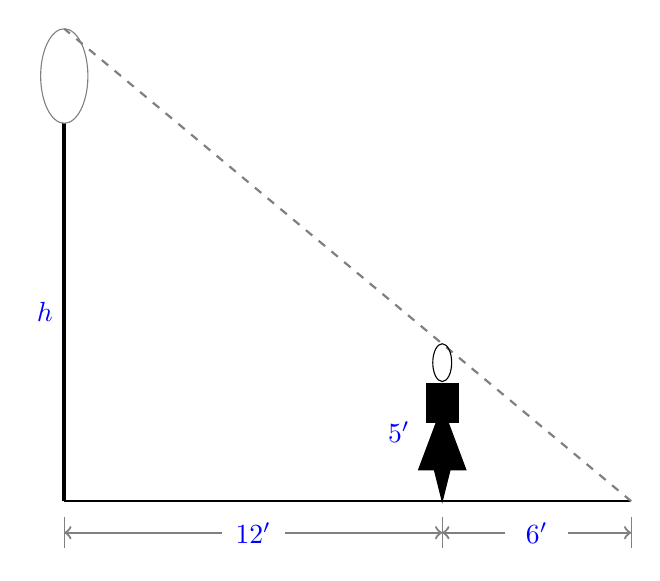
\begin{tikzpicture}[scale=2]

\coordinate (A) at (0,0);
\coordinate (B) at (-1.2,1);
\coordinate (C) at (-1.2,0);
\coordinate (D) at (-3.6,3);
\coordinate (E) at (-3.6,0);

\draw[black,  thick] (A) --  (C) node[below,midway, yshift=-4] {\color{blue}$6'$} ;
\draw[white,  thick] (-1.2,.7) -- (C) node[left, midway, xshift=-8,yshift=5] {\color{blue}$5'$} ;
\draw[black,  thick] (C) -- (E) node[below, midway, yshift=-4] {\color{blue}$12'$} ;
\draw[black,  ultra thick] (-3.6,2.4) -- (E) node[left, midway,yshift=0] {\color{blue}$h$} ;
\draw[gray,  thick, dashed] (A) -- (D)  ;

\draw [gray] (-3.6,2.7) ellipse (.15 and .3);
\draw [black] (-1.2,.88) ellipse (.06 and .12);
\filldraw[black] (-1.1,.75) rectangle +(-.2,-.25);
\filldraw[black] (-1.2,.6) -- (-1.35,.2) -- (-1.05,.2) --cycle;
\filldraw[black] (-1.2,0) -- (-1.25,.2) -- (-1.15,.2) --cycle;

\draw[gray] (-3.6, -.1) -- +(0,-.2);
\draw[gray] (-1.2, -.1) -- +(0,-.2);
\draw[gray] (0, -.1) -- +(0,-.2);
\draw[gray, thick, <-] (0, -.2) -- +(-.4,0);
\draw[gray, thick, <-] (-1.2, -.2) -- +(.4,0);
\draw[gray, thick, <-] (-3.6, -.2) -- +(1,0);
\draw[gray, thick, <-] (-1.2, -.2) -- +(-1,0);

\end{tikzpicture}
\newline



Study question 4
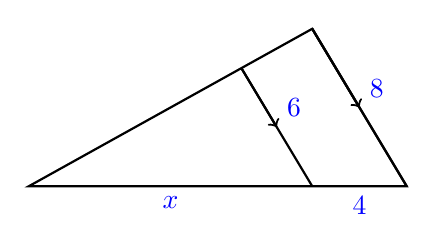
\begin{tikzpicture}

\coordinate (A) at (0,0);
\coordinate (B) at (3.6,0);
\coordinate (C) at (2.7,1.5);
\coordinate (D) at (4.8,0);
\coordinate (E) at (3.6,2);

\draw[black, thick] (A)--(D)--(E)--cycle;
\draw[black, thick] (A) -- (B) node [below, midway] {\color{blue}$x$};
\draw[black, thick] (D) -- (B) node [below, midway] {\color{blue}$4$};
\draw[black, thick] (D) -- (E) node [above right, midway] {\color{blue}$8$};
\draw[black, thick] (C) -- (B) node [above right, midway] {\color{blue}$6$};

\draw[black,  thick, ->] (C) --  (3.15,.75)  ;
\draw[black,  thick, ->] (E) --  (4.2,1)  ;

\end{tikzpicture}
\newline


Hmwk 1.2.1
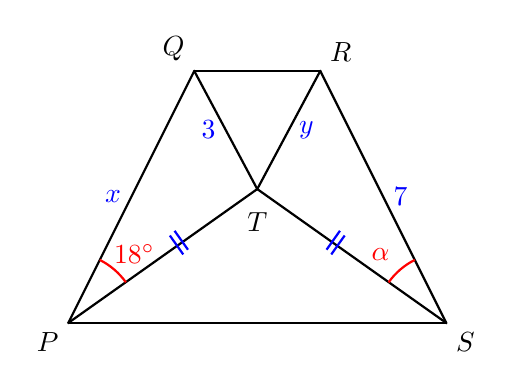
\begin{tikzpicture}

\coordinate (T) at (0,0);
\coordinate (P) at (-2.4,-1.7);
\coordinate (Q) at (-.8,1.5);
\coordinate (R) at (.8,1.5);
\coordinate (S) at (2.4,-1.7);

\filldraw [black] (T) circle (.2pt) node[anchor=north,yshift=-5] {$T$};
\filldraw [black] (P) circle (.2pt) node[anchor=north east,yshift=0] {$P$};
\filldraw [black] (Q) circle (.2pt) node[anchor=south east,yshift=0] {$Q$};
\filldraw [black] (R) circle (.2pt) node[anchor=south west,yshift=0] {$R$};
\filldraw [black] (S) circle (.2pt) node[anchor=north west,yshift=0] {$S$};

\draw[black, thick] (P)--(S);
\draw[black, thick] (Q)--(R);
\draw[black, thick] (P)--(T);
\draw[black, thick] (T)--(S);
\draw[black, thick] (P) -- (Q) node [left, midway] {\color{blue}$x$};
\draw[black, thick] (R) -- (S) node [right, midway] {\color{blue}$7$};
\draw[black, thick] (Q) -- (T) node [left, midway] {\color{blue}$3$};
\draw[black, thick] (R) -- (T) node [ right, midway] {\color{blue}$y$};
\draw[blue, thick] (-.94,-.83)-- +(-.17,.24);
\draw[blue, thick] (-.88,-.77)-- +(-.17,.24);
\draw[blue, thick] (.94,-.83)-- +(.17,.24);
\draw[blue, thick] (.88,-.77)-- +(.17,.24);

\draw [red,thick] (-2.,-0.9) arc({atan(2)}:{atan(17/24)}:.9) node[above right,xshift=-8,yshift=3] {$18\degree$};
\draw [red,thick] (2.,-0.9) arc({180-atan(2)}:{180-atan(17/24)}:.9) node[above left,xshift=4,yshift=4] {$\alpha$};

\end{tikzpicture}
\newline



Hmwk 1.2.2
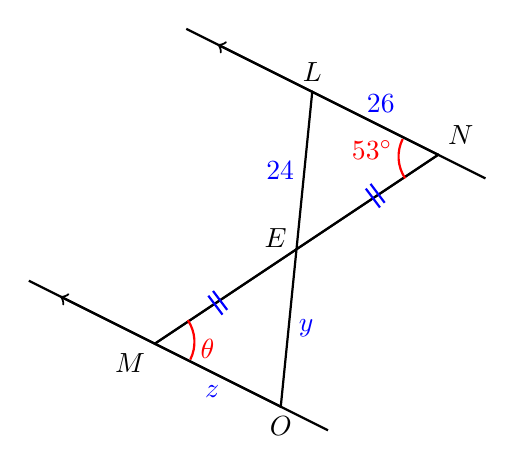
\begin{tikzpicture}

\coordinate (E) at (0,0);
\coordinate (M) at (-1.8,-1.2);
\coordinate (N) at (1.8,1.2);
\coordinate (L) at (.2,2);
\coordinate (O) at (-.2,-2);

\filldraw [black] (E) circle (.2pt) node[anchor=east,yshift=4] {$E$};
\filldraw [black] (M) circle (.2pt) node[anchor=north east,yshift=0] {$M$};
\filldraw [black] (N) circle (.2pt) node[anchor=south west,yshift=0] {$N$};
\filldraw [black] (L) circle (.2pt) node[anchor=south,yshift=0] {$L$};
\filldraw [black] (O) circle (.2pt) node[anchor=north ,yshift=0] {$O$};

\draw[black, thick] (M)--(N);
\draw[black, thick] (M)--(N);
\draw[black, thick] (E) -- (L) node [left, midway] {\color{blue}$24$};
\draw[black, thick] (E) -- (O) node [right, midway] {\color{blue}$y$};
\draw[black, thick] (M) -- (O) node [below, midway,xshift=-2] {\color{blue}$z$};
\draw[black, thick] (L) -- (N) node [ above, midway,xshift=2] {\color{blue}$26$};
\draw[blue, thick] (-.94,-.83)-- +(-.18,.24);
\draw[blue, thick] (-.88,-.77)-- +(-.18,.24);
\draw[blue, thick] (.94,.83)-- +(.18,-.24);
\draw[blue, thick] (.88,.77)-- +(.18,-.24);

\coordinate (M2) at (-3,-0.6);
\coordinate (N2) at (2.4,0.9);
\coordinate (M3) at (-3.4,-0.4);
\coordinate (L3) at (-1.4,2.8);
\coordinate (L2) at (-1,2.6);
\coordinate (O2) at (0.4,-2.3);

\draw[black, thick, <-] (M2)--(O2);
\draw[black, thick, <-] (L2)--(N2);
\draw[black, thick] (M)--(M3);
\draw[black, thick] (L3)--(L);

\draw [red,thick] (-1.38,-0.9) arc({atan(2/3)}:{atan(-.5)}:.5) node[ right,xshift=0,yshift=4] {$\theta$};
\draw [red,thick] (1.38,0.9) arc({180+atan(2/3)}:{180+atan(-.5)}:.5) node[ left,xshift=0,yshift=-4] {$53\degree$};

\end{tikzpicture}
\newline



Hmwk 1.2.3
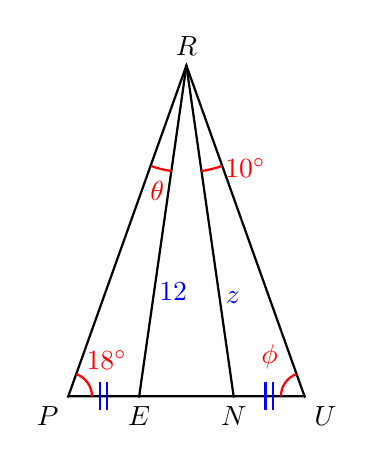
\begin{tikzpicture}[scale=1.5]

\coordinate (R) at (0,0);
\coordinate (P) at (-1.,-2.8);
\coordinate (U) at (1, -2.8);
\coordinate (E) at (-.4,-2.8);
\coordinate (N) at (.4,-2.8);

\filldraw [black] (R) circle (.2pt) node[anchor=south] {$R$};
\filldraw [black] (P) circle (.2pt) node[anchor=north east,yshift=0] {$P$};
\filldraw [black] (U) circle (.2pt) node[anchor=north west,yshift=0] {$U$};
\filldraw [black] (E) circle (.2pt) node[anchor=north ,yshift=0] {$E$};
\filldraw [black] (N) circle (.2pt) node[anchor=north,yshift=0] {$N$};

\draw[black, thick] (P)--(R)--(U)--cycle;
\draw[black, thick] (E) -- (R) node [below right, midway,xshift=-5,yshift=-15] {\color{blue}$12$};
\draw[black, thick] (R) -- (N) node [below right, midway,xshift=2,yshift=-18] {\color{blue}$z$};
\draw[blue, thick] (-.67,-2.92)-- +(0,.24);
\draw[blue, thick] (-.73,-2.92)-- +(0,.24);
\draw[blue, thick] (.67,-2.92)-- +(0,.24);
\draw[blue, thick] (.73,-2.92)-- +(0,.24);

\draw [red,thick] (-.8,-2.8) arc(0:{atan(2.8)}:.2) node[above right,xshift=0,yshift=-2] {$18\degree$};
\draw [red,thick] (.8,-2.8) arc(180:{180-atan(2.8)}:.2) node[above left,xshift=-3,yshift=-2] {$\phi$};
\draw [red,thick] (-.3,-.85) arc({180+atan(2.8)}:{180+atan(7)}:.9) node[below  left,xshift=1,yshift=0] {$\theta$};
\draw [red,thick] (.3,-.85) arc({-atan(2.8)}:{-atan(7)}:.9) node[  right,xshift=5,yshift=1] {$10\degree$};

\end{tikzpicture}
\newline


Hmwk 1.2.4
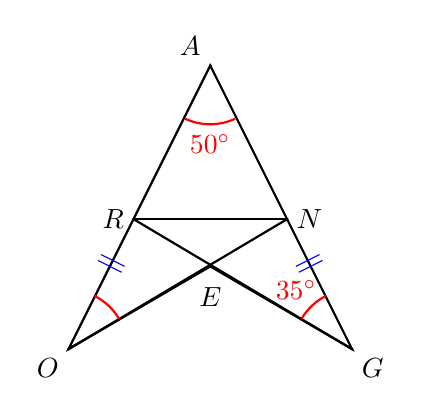
\begin{tikzpicture}[scale=1.5]

\coordinate (A) at (0,0);
\coordinate (R) at (-.65,-1.3);
\coordinate (N) at (.65, -1.3);
\coordinate (O) at (-1.2,-2.4);
\coordinate (G) at (1.2,-2.4);
\coordinate (E) at (0,-1.7);

\filldraw [black] (R) circle (.2pt) node[anchor=east] {$R$};
\filldraw [black] (N) circle (.2pt) node[anchor=west] {$N$};
\filldraw [black] (O) circle (.2pt) node[anchor=north east,yshift=0] {$O$};
\filldraw [black] (G) circle (.2pt) node[anchor=north west,yshift=0] {$G$};
\filldraw [black] (E) circle (.2pt) node[anchor=north ,yshift=-4] {$E$};
\filldraw [black] (A) circle (.2pt) node[anchor=south east,yshift=0] {$A$};

\draw[black, thick] (A)--(G)--(E)--(O)--cycle;
\draw[black, thick] (G) -- (R) ;
\draw[black, thick] (O)-- (N);
\draw[black, thick] (R)--(N);
\draw[blue] (-.95,-1.65)-- +(.2,-.1);
\draw[blue] (-.925,-1.6)-- +(.2,-.1);
\draw[blue] (.95,-1.65)-- +(-.2,-.1);
\draw[blue] (.925,-1.6)-- +(-.2,-.1);

\draw [red,thick] (-.98,-1.95) arc({atan(2)}:30.7:.5);
\draw [red,thick] (.98,-1.95) arc({180-atan(2)}:149.3:.5) node[above left,xshift=9,yshift=3] {$35\degree$};
\draw [red,thick] (.21,-.45) arc(-65:-115:.5) node[below, midway, xshift=0,yshift=0] {$50\degree$};

\end{tikzpicture}
\newline




Hmwk 1.2.7
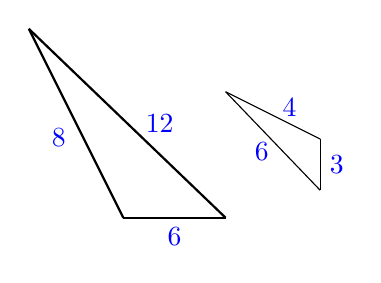
\begin{tikzpicture}

\coordinate (A) at (0,0);
\coordinate (B) at (-1.2,2.4);
\coordinate (C) at (1.3,0);

\draw[black,  thick] (A) --  (B) node[left,midway,yshift=-5]{\color{blue}$8$} ;
\draw[black,  thick] (C) --  (B) node[right,midway,xshift=3]{\color{blue}$12$} ;
\draw[black,  thick] (C) --  (A) node[below,midway]{\color{blue}$6$} ;


\draw[black, shift={(2.5 cm, 1 cm)}, rotate=90, scale=.5]  (0,0)--(1.2,2.4)  node[right,midway,yshift=3]{\color{blue}$4$};
\draw[black, shift={(2.5 cm, 1 cm)}, rotate=90, scale=.5]  (1.2,2.4)--(-1.3,0)  node[left,midway,xshift=2,yshift=-4]{\color{blue}$6$};
\draw[black, shift={(2.5 cm, 1 cm)}, rotate=90, scale=.5]  (0,0)--(-1.3,0) node[right,midway]{\color{blue}$3$}  ;

\end{tikzpicture}
\newline




Hmwk 1.2.8
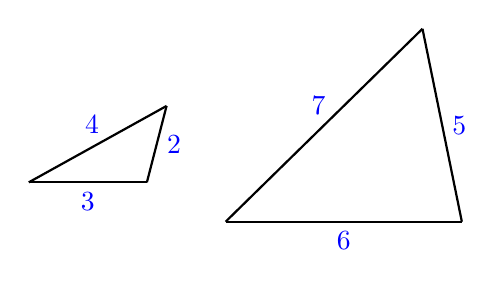
\begin{tikzpicture}

\coordinate (A) at (0,0);
\coordinate (B) at (1.75,.97);
\coordinate (C) at (1.5,0);

\draw[black,  thick] (A) --  (B) node[above,midway,xshift=-2]{\color{blue}$4$} ;
\draw[black,  thick] (C) --  (B) node[right,midway,xshift=0]{\color{blue}$2$} ;
\draw[black,  thick] (C) --  (A) node[below,midway]{\color{blue}$3$} ;

\coordinate (A2) at (2.5,-.5);
\coordinate (B2) at (5,1.95);
\coordinate (C2) at (5.5,-.5);

\draw[black,  thick] (A2) --  (B2) node[above,midway,xshift=-2]{\color{blue}$7$} ;
\draw[black,  thick] (C2) --  (B2) node[right,midway,xshift=0]{\color{blue}$5$} ;
\draw[black,  thick] (C2) --  (A2) node[below,midway]{\color{blue}$6$} ;

\end{tikzpicture}
\newline




Hmwk 1.2.9
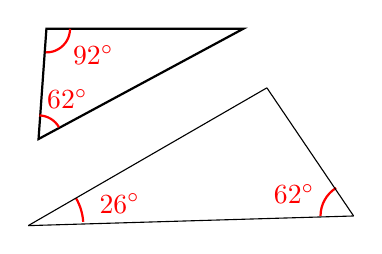
\begin{tikzpicture}

\coordinate (A) at (0,0);
\coordinate (B) at (-.1,-1.4);
\coordinate (C) at (2.5,0);

\draw[black,  thick] (A) --  (B) -- (C) -- cycle ;
\draw[red, thick] (0.16,-1.25) arc (30:88:0.3) node [above right, midway, xshift=-5, yshift=0] {\color{red}$62\degree$};
\draw[red, thick] (.3,0) arc (0:-92:0.3) node [below right, midway, xshift=0, yshift=4] {\color{red}$92\degree$};

\draw[red, thick,shift={(2.8 cm, -.75 cm)}, rotate=30, scale=1.4]  (-0.16,-1.25) arc (150:92:0.3) node [above left, midway, xshift=0, yshift=-5] {\color{red}$62\degree$};
\draw[red, thick, shift={(2.8 cm, -.75 cm)}, rotate=30, scale=1.4] (-2.0,0) arc (0:-26:0.5) node [above right, midway, xshift=3, yshift=-5] {\color{red}$26\degree$};

\draw[black, shift={(2.8 cm, -.75 cm)}, rotate=30, scale=1.4]  (0,0)--(.1,-1.4);
\draw[black, shift={(2.8 cm, -.75 cm)}, rotate=30, scale=1.4]  (.1,-1.4)--(-2.5,0) ;
\draw[black, shift={(2.8 cm, -.75 cm)}, rotate=30, scale=1.4]  (0,0)--(-2.5,0) ;

\end{tikzpicture}
\newline


Hmwk 1.2.10
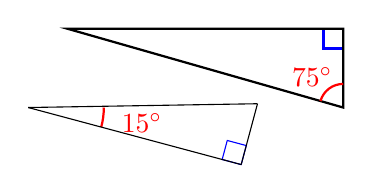
\begin{tikzpicture}

\coordinate (A) at (0,0);
\coordinate (B) at (3.5,-1);
\coordinate (C) at (3.5,0);

\draw[blue, thick] (C) rectangle +(-.25,-.25);
\draw[black,  thick] (A) --  (B) -- (C) -- cycle ;
\draw[red, thick] (3.5,-.7) arc (90:{180-atan(1/3.5)}:0.3) node [above left, midway, xshift=5, yshift=-3] {\color{red}$75\degree$};

\draw[red, thick, shift={(-.5 cm, -1 cm)}, rotate=-15, scale=0.8] (1.2,0) arc (0:15:1.2) node [ right, midway, xshift=3, yshift=-2] {\color{red}$15\degree$};

\draw[blue, shift={(-.5 cm, -1 cm)}, rotate=-15, scale=0.8]  (3.5,0) rectangle +(-.3125,.3125);
\draw[black, shift={(-.5 cm, -1 cm)}, rotate=-15, scale=0.8]  (0,0)--(3.5,1);
\draw[black, shift={(-.5 cm, -1 cm)}, rotate=-15, scale=0.8]  (3.5,1)--(3.5,0) ;
\draw[black, shift={(-.5 cm, -1 cm)}, rotate=-15, scale=0.8]  (0,0)--(3.5,0) ;

\end{tikzpicture}
\newline



Hmwk 1.2.11
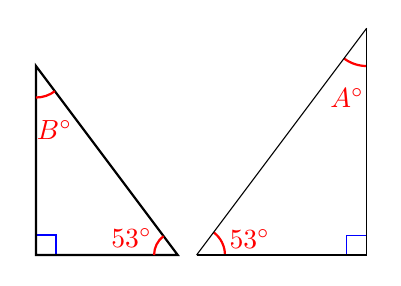
\begin{tikzpicture}

\coordinate (O) at (0,0);
\coordinate (B) at (0,2.4);
\coordinate (C) at (1.8,0);

\draw[blue, thick] (O) rectangle +(.25,.25);
\draw[black,  thick] (O) --  (B) -- (C) -- cycle ;
\draw[red, thick] (0,2) arc (-90:{atan(-4/3)}:0.4) node [below right, midway, xshift=-7, yshift=-5] {\color{red}$B\degree$};
\draw[red, thick] (1.5,0) arc (180:127:0.3) node [above left, midway, xshift=2, yshift=-5] {\color{red}$53\degree$};

\draw[red, thick, shift={(4.2 cm, 0 cm)}, scale=1.2]  (0,2) arc (-90:{atan(4/3)-180}:0.4) node [below left, midway, xshift=7, yshift=-5] {\color{red}$A\degree$};
\draw[red, thick, shift={(4.2 cm, 0 cm)}, scale=1.2] (-1.5,0) arc (0:53:0.3) node [above right, midway, xshift=-1, yshift=-6] {\color{red}$53\degree$};
\draw[blue, shift={(4.2 cm, 0 cm)}, scale=1.2]  (0,0) rectangle +(-.21,.21);
\draw[black, shift={(4.2 cm, 0 cm)}, scale=1.2]  (0,0)--(0,2.4);
\draw[black, shift={(4.2 cm, 0 cm)}, scale=1.2]  (0,2.4)--(-1.8,0) ;
\draw[black, shift={(4.2 cm, 0 cm)},  scale=1.2]  (0,0)--(-1.8,0) ;

\end{tikzpicture}
\newline


Hmwk 1.2.12
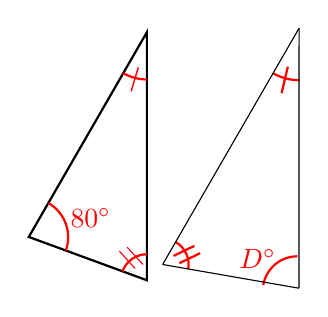
\begin{tikzpicture}

\coordinate (O) at (0,0);
\coordinate (B) at (-1.5,.55);
\coordinate (C) at (0,3.15);

\draw[black,  thick] (O) --  (B) -- (C) -- cycle ;
\draw[red, thick] (0,2.55) arc (-90:{atan(2.6/1.5)-180}:0.6);
\draw[red, thick] (0,.33) arc (90:{180-atan(.55/1.5)}:0.33);
\draw[red, thick] (-1.25,.98) arc (60:-20:0.5) node [right, midway, xshift=-2, yshift=2] {\color{red}$80\degree$};
\draw[red] (-.2,2.4) -- +(.09,.3);
\draw[red] (-.2,2.4) -- +(.09,.3);

\draw[red] (-.15,.15) -- +(-.2,.22);
\draw[red] (-.05,.20) -- +(-.2,.22);

\draw[red, thick, shift={(.2 cm, .2 cm)}, rotate=-30, scale=1.1] (.2,2.4) -- +(-.09,.3);
\draw[red, thick, shift={(.2 cm, .2 cm)}, rotate=-30, scale=1.1] (.16,.11) -- +(.15,.22);
\draw[red, thick, shift={(.2 cm, .2 cm)}, rotate=-30, scale=1.1] (.06,.15) -- +(.15,.22);


\draw[red, thick, shift={(.2 cm, .2 cm)}, rotate=-30, scale=1.1]  (0,2.55) arc (-90:{-atan(2.6/1.5)}:0.6) ;
\draw[red, thick, shift={(.2 cm, .2 cm)}, rotate=-30, scale=1.1] (0,.3) arc (90:{atan(.55/1.5)}:0.3);
\draw[red, thick, shift={(.2 cm, .2 cm)}, rotate=-30, scale=1.1] (1.3,.86) arc (120:200:0.4)  node [left, midway, xshift=4, yshift=2] {\color{red}$D\degree$};

\draw[black, shift={(.2 cm, .2 cm)}, rotate=-30, scale=1.1]  (0,0)--(1.5,.55);
\draw[black, shift={(.2 cm, .2 cm)}, rotate=-30, scale=1.1]  (1.5,.55)--(0,3.15) ;
\draw[black, shift={(.2 cm, .2 cm)},  rotate=-30, scale=1.1]  (0,0)--(0,3.15) ;

\end{tikzpicture}
\newline



Hmwk 1.2.13
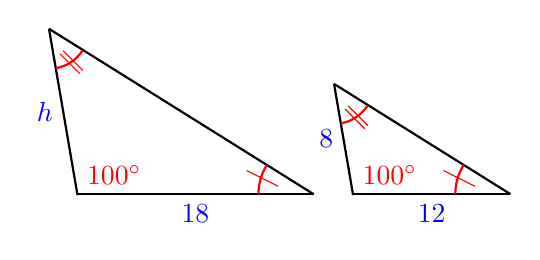
\begin{tikzpicture}

\coordinate (O) at (0,0);
\coordinate (B) at (-.36,2.1);
\coordinate (C) at (3,0);

\draw[black,  thick] (O) --  (B) node[left,midway] {\color{blue}$h$} ;
\draw[black,  thick]  (B) -- (C)  ;
\draw[black,  thick] (O) --  (C)   node[below,midway] {\color{blue}$18$};

\draw[red, thick] (2.3,0) arc (180:{180-atan(2.1/3.356)}:0.7);
\filldraw[black] (O) circle(.2pt) node[anchor= south west] {\color{red}$100\degree$};
\draw[red] (2.55,0.1) -- +(-.4,.2);

\draw[red, thick] (-.27,1.6) arc (280:{360-atan(2.1/3.356)}:0.5);
\draw[red] (-.22,1.78) -- +(.25,-.25);
\draw[red] (-.18,1.82) -- +(.25,-.25);

\coordinate (O2) at (3.5,0);
\coordinate (B2) at (3.26,1.4);
\coordinate (C2) at (5.5,0);
\draw[black,  thick] (O2) --  (B2) node[left,midway] {\color{blue}$8$} ;
\draw[black,  thick]  (B2) -- (C2)  ;
\draw[black,  thick] (O2) --  (C2)   node[below,midway] {\color{blue}$12$};

\draw[red, thick] (4.8,0) arc (180:{180-atan(2.1/3.356)}:0.7);
\filldraw[black] (O2) circle(.2pt) node[anchor= south west] {\color{red}$100\degree$};
\draw[red] (5.05,0.1) -- +(-.4,.2);

\draw[red, thick] (3.35,.9) arc (280:{360-atan(2.1/3.356)}:0.5);
\draw[red] (3.40,1.08) -- +(.25,-.25);
\draw[red] (3.44,1.12) -- +(.25,-.25);

\end{tikzpicture}
\newline



Hmwk 1.2.14
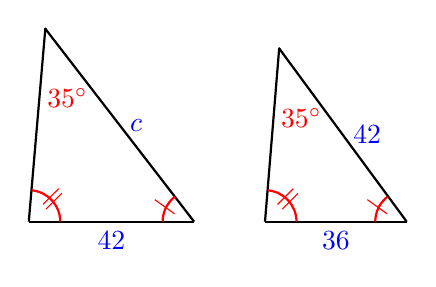
\begin{tikzpicture}

\coordinate (O) at (0,0);
\coordinate (B) at (0.21,2.45);
\coordinate (C) at (2.1,0);

\draw[black,  thick] (O) --  (B) ;
\draw[black,  thick]  (B) -- (C)   node[right,midway] {\color{blue}$c$};
\draw[black,  thick] (O) --  (C)   node[below,midway] {\color{blue}$42$};

\draw[red, thick] (0.4,0) arc (0:85:0.4);
\filldraw[black] (B) circle(.2pt) node[anchor= north,xshift=8,yshift=-18] {\color{red}$35\degree$};
\draw[red] (0.18,0.22) -- +(.2,.2);
\draw[red] (0.22,0.16) -- +(.2,.2);

\draw[red, thick] (1.7,0) arc (180:{180-atan(2.45/1.9)}:0.4);
\draw[red] (1.85,0.1) -- +(-.25,.18);

\coordinate (O2) at (3,0);
\coordinate (B2) at (3.18,2.2);
\coordinate (C2) at (4.8,0);
\draw[black,  thick] (O2) --  (B2) ;
\draw[black,  thick]  (B2) -- (C2)   node[right,midway] {\color{blue}$42$};;
\draw[black,  thick] (O2) --  (C2)   node[below,midway] {\color{blue}$36$};

\draw[red, thick] (3.4,0) arc (0:85:0.4);
\filldraw[black] (B2) circle(.2pt) node[anchor= north,xshift=8,yshift=-18] {\color{red}$35\degree$};
\draw[red] (3.16,0.22) -- +(.2,.2);
\draw[red] (3.22,0.16) -- +(.2,.2);

\draw[red, thick] (4.4,0) arc (180:{180-atan(2.45/1.9)}:0.4);
\draw[red] (4.55,0.1) -- +(-.25,.18);

\end{tikzpicture}
\newline



Hmwk 1.2.15
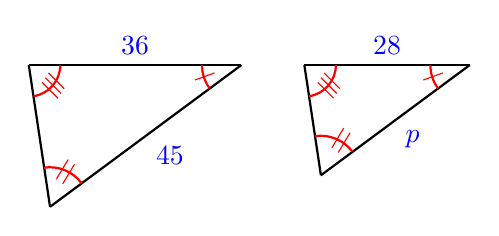
\begin{tikzpicture}

\coordinate (O) at (0,0);
\coordinate (B) at (0.27,-1.8);
\coordinate (C) at (2.7,0);

\draw[black,  thick] (O) --  (B) ;
\draw[black,  thick]  (B) -- (C)   node[below right,midway] {\color{blue}$45$};
\draw[black,  thick] (O) --  (C)   node[above,midway] {\color{blue}$36$};

\draw[red, thick] (0.4,0) arc (0:{atan(-20/3)}:0.4);
\draw[red] (0.17,-0.22) -- +(.2,-.2);
\draw[red] (0.21,-0.16) -- +(.2,-.2);
\draw[red] (0.25,-0.10) -- +(.2,-.2);

\draw[red, thick] (2.2,0) arc (180:{180+atan(1.8/2.43)}:0.5);
\draw[red] (2.36,-0.1) -- +(-.25,-.09);

\draw[red, thick] (0.67,-1.5) arc ({atan(1.8/2.43)}:{180-atan(20/3}:0.5);
\draw[red] (0.35,-1.45) -- +(.15,.25);
\draw[red] (0.43,-1.51) -- +(.15,.25);

\coordinate (O2) at (3.5,0);
\coordinate (B2) at (3.71,-1.4);
\coordinate (C2) at (5.6,0);
\draw[black,  thick] (O2) --  (B2) ;
\draw[black,  thick]  (B2) -- (C2)   node[below right,midway] {\color{blue}$p$};;
\draw[black,  thick] (O2) --  (C2)   node[above,midway] {\color{blue}$28$};

\draw[red, thick] (3.9,0) arc (0:{atan(-20/3)}:0.4);
\draw[red] (3.67,-0.22) -- +(.2,-.2);
\draw[red] (3.71,-0.16) -- +(.2,-.2);
\draw[red] (3.75,-0.10) -- +(.2,-.2);

\draw[red, thick] (5.1,0) arc (180:{180+atan(1.8/2.43)}:0.5);
\draw[red] (5.26,-0.1) -- +(-.25,-.09);

\draw[red, thick] (4.11,-1.1) arc ({atan(1.8/2.43)}:{180-atan(20/3}:0.5);
\draw[red] (3.85,-1.05) -- +(.15,.25);
\draw[red] (3.93,-1.11) -- +(.15,.25);

\end{tikzpicture}
\newline



Hmwk 1.2.16
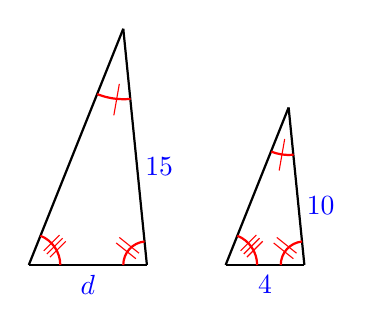
\begin{tikzpicture}

\coordinate (O) at (0,0);
\coordinate (B) at (1.2,3);
\coordinate (C) at (1.5,0);

\draw[black,  thick] (O) --  (B) ;
\draw[black,  thick]  (B) -- (C)   node[below right,midway] {\color{blue}$15$};
\draw[black,  thick] (O) --  (C)   node[below,midway] {\color{blue}$d$};

\draw[red, thick] (0.4,0) arc (0:{atan(3/1.2)}:0.4);
\draw[red] (0.19,0.18) -- +(.2,.2);
\draw[red] (0.23,0.14) -- +(.2,.2);
\draw[red] (0.27,0.10) -- +(.2,.2);

\draw[red, thick] (0.87,2.17) arc ({180+atan(3/1.2)}:{360-atan(10)}:0.9);
\draw[red] (1.15,2.3) -- +(-.07,-.4);

\draw[red, thick] (1.2,0) arc (180:{180-atan(10}:0.3);
\draw[red] (1.4,0.15) -- +(-.25,.20);
\draw[red] (1.36,0.08) -- +(-.25,.20);

\coordinate (O2) at (2.5,0);
\coordinate (B2) at (3.3,2);
\coordinate (C2) at (3.5,0);
\draw[black,  thick] (O2) --  (B2) ;
\draw[black,  thick]  (B2) -- (C2)   node[below right,midway] {\color{blue}$10$};;
\draw[black,  thick] (O2) --  (C2)   node[below,midway] {\color{blue}$4$};

\draw[red, thick] (2.9,0) arc (0:{atan(3/1.2)}:0.4);
\draw[red] (2.69,0.18) -- +(.2,.2);
\draw[red] (2.73,0.14) -- +(.2,.2);
\draw[red] (2.77,0.10) -- +(.2,.2);

\draw[red, thick] (3.08,1.44) arc ({180+atan(3/1.2)}:{360-atan(10)}:0.6);
\draw[red] (3.25,1.6) -- +(-.07,-.4);

\draw[red, thick] (3.2,0) arc (180:{180-atan(10}:0.3);
\draw[red] (3.4,0.15) -- +(-.25,.20);
\draw[red] (3.36,0.08) -- +(-.25,.20);

\end{tikzpicture}
\newline




Hmwk 1.2.17
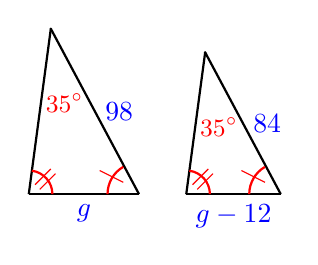
\begin{tikzpicture}

\coordinate (O) at (0,0);
\coordinate (B) at (.28,2.1);
\coordinate (C) at (1.4,0);

\draw[black,  thick] (O) --  (B) ;
\draw[black,  thick]  (B) -- (C) node[right,midway] {\color{blue}$98$};
\draw[black,  thick] (O) --  (C)   node[below,midway] {\color{blue}$g$};

\draw[red, thick] (1,0) arc (180:{180-atan(2.1/1.22)}:0.4);
\filldraw[black] (B) circle(.2pt) node[anchor= north, xshift=5,yshift=-20] {\small\color{red}$35\degree$};
\draw[red] (1.2,0.15) -- +(-.3,.15);

\draw[red, thick] (.3,0) arc (0:{atan(2.1/.28)}:0.3);
\draw[red] (.14,.06) -- +(.20,.20);
\draw[red] (.08,.12) -- +(.20,.20);

\coordinate (O2) at (2,0);
\coordinate (B2) at (2.24,1.8);
\coordinate (C2) at (3.2,0);
\draw[black,  thick] (O2) --  (B2) ;
\draw[black,  thick]  (B2) -- (C2) node[right,midway] {\color{blue}$84$} ;
\draw[black,  thick] (O2) --  (C2)   node[below,midway] {\color{blue}$g-12$};

\draw[red, thick] (2.8,0) arc (180:{180-atan(2.1/1.22)}:0.4);
\filldraw[black] (B2) circle(.2pt) node[anchor= north, xshift=5,yshift=-20] {\small\color{red}$35\degree$};
\draw[red] (3,0.15) -- +(-.3,.15);

\draw[red, thick] (2.3,0) arc (0:{atan(2.1/.28)}:0.3);
\draw[red] (2.14,.06) -- +(.20,.20);
\draw[red] (2.08,.12) -- +(.20,.20);


\end{tikzpicture}
\newline






Hmwk 1.2.18
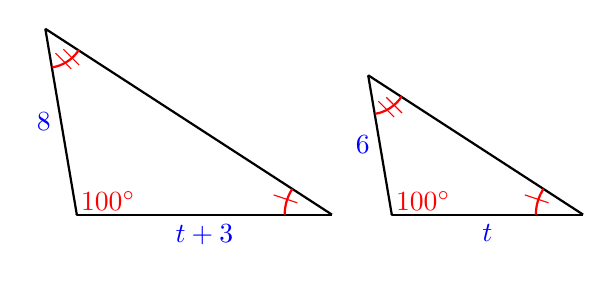
\begin{tikzpicture}

\coordinate (O) at (0,0);
\coordinate (B) at (-.4,2.36);
\coordinate (C) at (3.24,0);

\draw[black,  thick] (O) --  (B)  node[left,midway] {\color{blue}$8$};
\draw[black,  thick]  (B) -- (C);
\draw[black,  thick] (O) --  (C)   node[below,midway] {\color{blue}$t+3$};

\filldraw[black] (O) circle(.2pt) node[anchor=south west, xshift=-2,yshift=-2] {\color{red}$100\degree$};
\draw[red, thick] (2.64,0) arc (180:{180-atan(2.36/3.64)}:0.6);
\draw[red] (2.8,0.15) -- +(-.3,.1);

\draw[red, thick] (-.31,1.87) arc ({-atan(5.9}:{-atan(2.36/3.64)}:0.5);
\draw[red] (-.27,2.05) -- +(.20,-.20);
\draw[red] (-.17,2.1) -- +(.20,-.20);

\coordinate (O2) at (4,0);
\coordinate (B2) at (3.7,1.77);
\coordinate (C2) at (6.43,0);
\draw[black,  thick] (O2) --  (B2) node[left,midway] {\color{blue}$6$};
\draw[black,  thick]  (B2) -- (C2)  ;
\draw[black,  thick] (O2) --  (C2)   node[below,midway] {\color{blue}$t$};

\filldraw[black] (O2) circle(.2pt) node[anchor=south west, xshift=-2,yshift=-2] {\color{red}$100\degree$};
\draw[red, thick] (5.83,0) arc (180:{180-atan(2.36/3.64)}:0.6);
\draw[red] (5.99,0.15) -- +(-.3,.1);

\draw[red, thick] (3.79,1.28) arc ({-atan(5.9}:{-atan(2.36/3.64)}:0.5);
\draw[red] (3.83,1.44) -- +(.20,-.20);
\draw[red] (3.93,1.49) -- +(.20,-.20);

\end{tikzpicture}
\newline



Hmwk 1.2.19
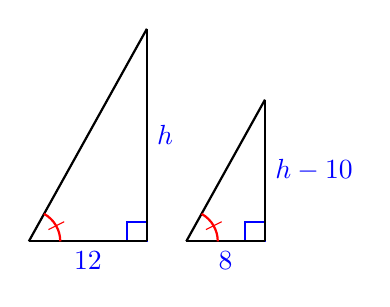
\begin{tikzpicture}

\coordinate (O) at (0,0);
\coordinate (B) at (1.5,2.7);
\coordinate (C) at (1.5,0);

\draw[blue, thick] (C) rectangle +(-.25,.25);
\draw[black,  thick] (O) --  (B) ;
\draw[black,  thick]  (B) -- (C)  node[right,midway] {\color{blue}$h$};
\draw[black,  thick] (O) --  (C)   node[below,midway] {\color{blue}$12$};

\draw[red, thick] (.4,0) arc (0:{atan(2.7/1.5)}:0.4);
\draw[red] (.25,0.15) -- +(.2,.1);


\coordinate (O2) at (2,0);
\coordinate (B2) at (3,1.8);
\coordinate (C2) at (3,0);
\draw[blue, thick] (C2) rectangle +(-.25,.25);
\draw[black,  thick] (O2) --  (B2);
\draw[black,  thick]  (B2) -- (C2)    node[right,midway] {\color{blue}$h-10$};
\draw[black,  thick] (O2) --  (C2)   node[below,midway] {\color{blue}$8$};

\draw[red, thick] (2.4,0) arc (0:{atan(2.7/1.5)}:0.4);
\draw[red] (2.25,0.15) -- +(.2,.1);

\end{tikzpicture}
\newline


Hmwk 1.2.20
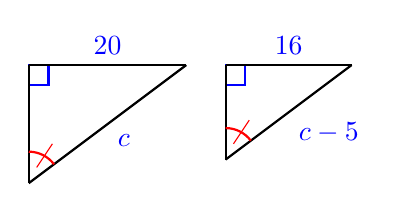
\begin{tikzpicture}

\coordinate (O) at (0,0);
\coordinate (B) at (2,0);
\coordinate (C) at (0,-1.5);

\draw[blue, thick] (O) rectangle +(.25,-.25);
\draw[black,  thick] (O) --  (B)   node[above,midway] {\color{blue}$20$};
\draw[black,  thick]  (B) -- (C)  node[below right,midway] {\color{blue}$c$};
\draw[black,  thick] (O) --  (C) ;

\draw[red, thick] (0,-1.1) arc (90:{atan(.75)}:0.4);
\draw[red] (.1,-1.3) -- +(.2,.3);


\coordinate (O2) at (2.5,0);
\coordinate (B2) at (4.1,0);
\coordinate (C2) at (2.5,-1.2);
\draw[blue, thick] (O2) rectangle +(.25,-.25);
\draw[black,  thick] (O2) --  (B2)   node[above,midway] {\color{blue}$16$};
\draw[black,  thick]  (B2) -- (C2)    node[below right,midway] {\color{blue}$c-5$};
\draw[black,  thick] (O2) --  (C2)  ;

\draw[red, thick] (2.5,-0.8) arc (90:{atan(.75)}:0.4);
\draw[red] (2.6,-1) -- +(.2,.3);


\end{tikzpicture}
\newline

hp1-2-21 through hp1-2-38 clipped from intro algebra pdf document



Hmwk 1.2.39
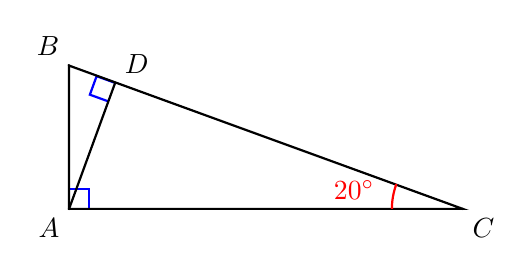
\begin{tikzpicture}

\coordinate (A) at (0,0);
\coordinate (B) at (0,1.82);
\coordinate (C) at (5,0);
\coordinate (D) at (.585,1.6);

\draw[blue, thick] (A) rectangle +(.25,.25);
\draw[blue,thick] (D) -- ++(-.235,.0855) -- ++(-.0855,-.235) -- ++(.235,-.0855);
\draw[black,  thick] (A) --  (B) --(C)--cycle;
\draw[black,  thick] (A) --  (D) ;

\draw[red, thick] (4.1,0) arc (180:{180-atan(1.5/4)}:0.9) node [above left, midway, xshift=-3,yshift=-5] {$20\degree$};
\filldraw [black] (A) circle (.2pt) node[anchor=north east] {$A$};
\filldraw [black] (B) circle (.2pt) node[anchor=south east] {$B$};
\filldraw [black] (C) circle (.2pt) node[anchor=north west] {$C$};
\filldraw [black] (D) circle (.2pt) node[anchor=south west] {$D$};

\end{tikzpicture}
\newline



Hmwk 1.2.40
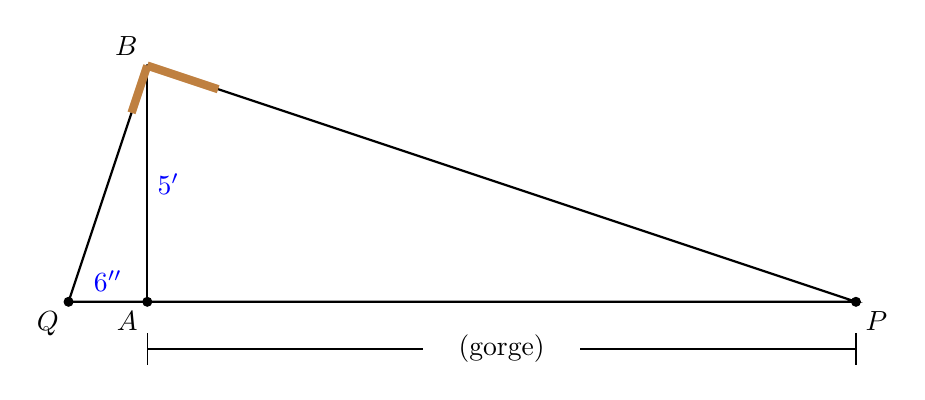
\begin{tikzpicture}

\coordinate (A) at (0,0);
\coordinate (B) at (0,3);
\coordinate (C) at (9,0);
\coordinate (Q) at (-1,0);

\draw[black,  thick] (A) --  (B) node[right, midway] {\color{blue}$5'$};
\draw[black,  thick] (A) --  (Q) node[above, midway] {\color{blue}$6''$};
\draw[black,  thick] (Q) --  (B) --(C)--cycle;

\filldraw [black] (A) circle (1.6pt) node[anchor=north east] {$A$};
\filldraw [black] (B) circle (.2pt) node[anchor=south east] {$B$};
\filldraw [black] (C) circle (1.6pt) node[anchor=north west] {$P$};
\filldraw [black] (Q) circle (1.6pt) node[anchor=north east] {$Q$};
\draw[brown,line width=3pt] (B) -- +(-.2,-.6);
\draw[brown,line width=3pt] (B) -- +(.9,-.3);

\draw[black,thin] (0,-.4) -- +(0,-.4);
\draw[black,thin] (9,-.4) -- +(0,-.4);
\draw[black,thin] (0,-.6) -- +(3.5,0);
\node at (4.5,-.6)  {(gorge)};
\draw[black,thin] (9,-.6) -- +(-3.5,0);


\end{tikzpicture}
\newline



Section 4.2 Angle of inclination
\begin{tikzpicture}

\coordinate (O) at (0,0);
\coordinate (x) at (3.5,0);
\coordinate (y) at (0,2);
\coordinate (A) at (3,1.8);
\coordinate (B) at (1.,0);
\coordinate (C) at (2.5,0);
\coordinate (D) at (-1,-1.8);

\draw[black,  thick, ->] (-1.5,0) --  (x) node[right] {$x$} ;
\draw[black,  thick, ->] (0,-2) --  (y) node[above] {$y$}  ;
\draw[black,  thick, <->] (D) --  (A)  ;
\draw[red, thick] (1.9,0) arc (0:{atan(0.9)}:.9) node [left, midway,xshift=0,yshift=-3] {$\alpha$};

\end{tikzpicture}
\newline

Section 4.2 Angle of inclination
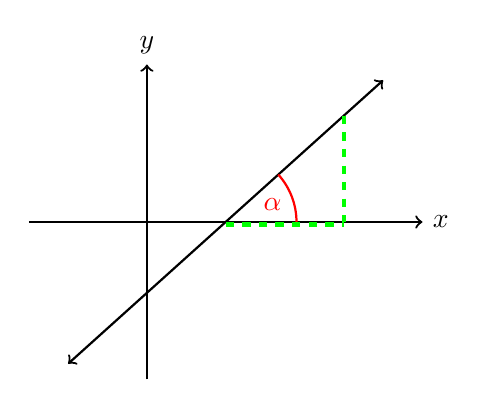
\begin{tikzpicture}

\coordinate (O) at (0,0);
\coordinate (x) at (3.5,0);
\coordinate (y) at (0,2);
\coordinate (A) at (3,1.8);
\coordinate (B) at (1.,0);
\coordinate (C) at (2.5,0);
\coordinate (D) at (-1,-1.8);

\draw[black,  thick, ->] (-1.5,0) --  (x) node[right] {$x$} ;
\draw[black,  thick, ->] (0,-2) --  (y) node[above] {$y$}  ;
\draw[black,  thick, <->] (D) --  (A)  ;
\draw[red, thick] (1.9,0) arc (0:{atan(0.9)}:.9) node [left, midway,xshift=0,yshift=-3] {$\alpha$};

\draw[green, ultra thick, dashed] (1,-.03) -- (2.5,-.03);
\draw[green, ultra thick, dashed] (2.5,1.35) -- (2.5,0);

\end{tikzpicture}
\newline


Exercise not used?
\begin{tikzpicture}
\coordinate (O) at (0,0);
\coordinate (A) at (0,0);
\coordinate (B) at (0,0);
\coordinate(C) at (0,0);
\coordinate (D) at (0,0);
\filldraw[black] (O) circle (.2pt) node[anchor=south west, xshift=6]{$50\degree$};
\filldraw[black] (A) circle (.2pt) node[anchor=south east]{$x$};
\filldraw[black] (B) circle (.2pt) node[anchor=north east, xshift=-6]{$y$};
\filldraw[black] (C) circle (.2pt) node[anchor=north west]{$z$};
%\draw[black,  thick] (A) -- (B) --( C) -- cycle;
\draw[black] (-2.3,0) --  (2.3,0);
\draw[black] (0.8,1.3) --  (-0.8,-1.3) ;
\end{tikzpicture}
\newline


\end{document}
